% This source file is part of the Geophysical Fluids Modeling Framework (GAME), which is released under the MIT license.
% Github repository: https://github.com/MHBalsmeier/game

\documentclass[10pt]{report}
\usepackage[utf8]{inputenc}
\usepackage{a4wide, amsmath, xcolor, longtable, geometry, fancyhdr, mathtools}
\usepackage[style = numeric, backend = biber]{biblatex}
\usepackage{fouriernc}
\usepackage[T1]{fontenc}
\usepackage[hidelinks]{hyperref}
\geometry{a4paper, top = 15mm, left = 5mm, right = 5mm, bottom = 17mm}
\fancypagestyle{plain}{
\fancyhead[L]{\texttt{GAME} documentation}
\fancyhead[R]{\textsc{\texttt{GAME} development team}}
\fancyfoot[C]{\thepage}
\addtolength\footskip{12pt}}
\definecolor{table_green}{rgb}{0, 0.6, 0}
\title{\texttt{Geophysical Fluids Modeling Framework} Documentation}
\author{\texttt{GAME} Development Team}
\date{}
\newcommand{\md}[1]{\frac{D#1}{Dt}}
\newcommand{\omegabi}{\text{{\osgbi ω}}}
\newcommand{\mubi}{\text{{\osgbi μ}}}
\newcommand{\sigmabi}{\text{{\osgbi σ}}}
\newcommand{\epsilonbi}{\text{{\osgbi ϵ}}}
\newcommand{\etabi}{\text{{\osgbi η}}}
\newcommand{\zetabi}{\text{{\osgbi ζ}}}
\addbibresource{references.bib}
\DeclareFieldFormat[article]{title}{{#1}}

\begin{document}

\maketitle
\tableofcontents

\chapter{Introduction}
\label{chap:introduction}

The \texttt{Geophysical Fluids Modeling Framework (GAME)} is a non-hydrostatic hexagonal C grid dynamical core with the possibility to advect a variable number of constituents. The term \textit{dynamical core} typically refers to the simulation of a dry atmosphere. Everything else is then referred to as \textit{physics}. Diffusive terms, including turbulence parameterizations, are sometimes understood to be part of the dynamical core and sometimes seen as part of the model's physics. The dry air is in this understanding a "carrier medium", whereas constituents, including water in different phases, are usually only passively advected. This thinking always leads to deep physical inconsistencies during later stages of model development, whose impact on forecast and climate simulation accuracy remains unknown.

Therefore, a new, capaple framework for simulating geophysical fluids is necessary and, due to the advent of even more powerful computers, also realistic. The \texttt{GAME} can be seen as a dynamical core, but not in the traditional sense, instead rather in a modernized sense. Its aim is to simulate the dynamics of geophysical fluid flow accurately, and at the same time make it possible to couple the model to different constituents \textit{consistently}, which means without violating fundamental physical constraints. Following a modular way of thinking, the actual quantifications of the constituent's source terms have been split off into the \texttt{atmostracers} library \cite{atmostracers-github}, which is meant to evolve into a wide collection of source terms for atmospheric constituents, also including chemistry and parameterizations. For radiation, it is coupled to the \texttt{RTE+RRTMGP (Radiative Transfer for Energetics + Rapid and Accurate Radiative Transfer Model for Geophysical Circulation Model Applications—Parallel)} \cite{doi:10.1029/2019MS001621}, \cite{rte-rrtmgp-github} scheme, which follows a similar approach to radiation simulation as \texttt{GAME} follows to fluid simulation.

\chapter{Code structure}
\label{chap:code_structure}

The code of the model resides in the directory \texttt{core/src}. Every subdirectory in there, including \texttt{core/src} itself, contains a file named \texttt{info} containing information on the purpose and contents of this specific directory.

\chapter{Grid generation}
\label{chap:grid_generation}

\begin{figure}
\begin{center}
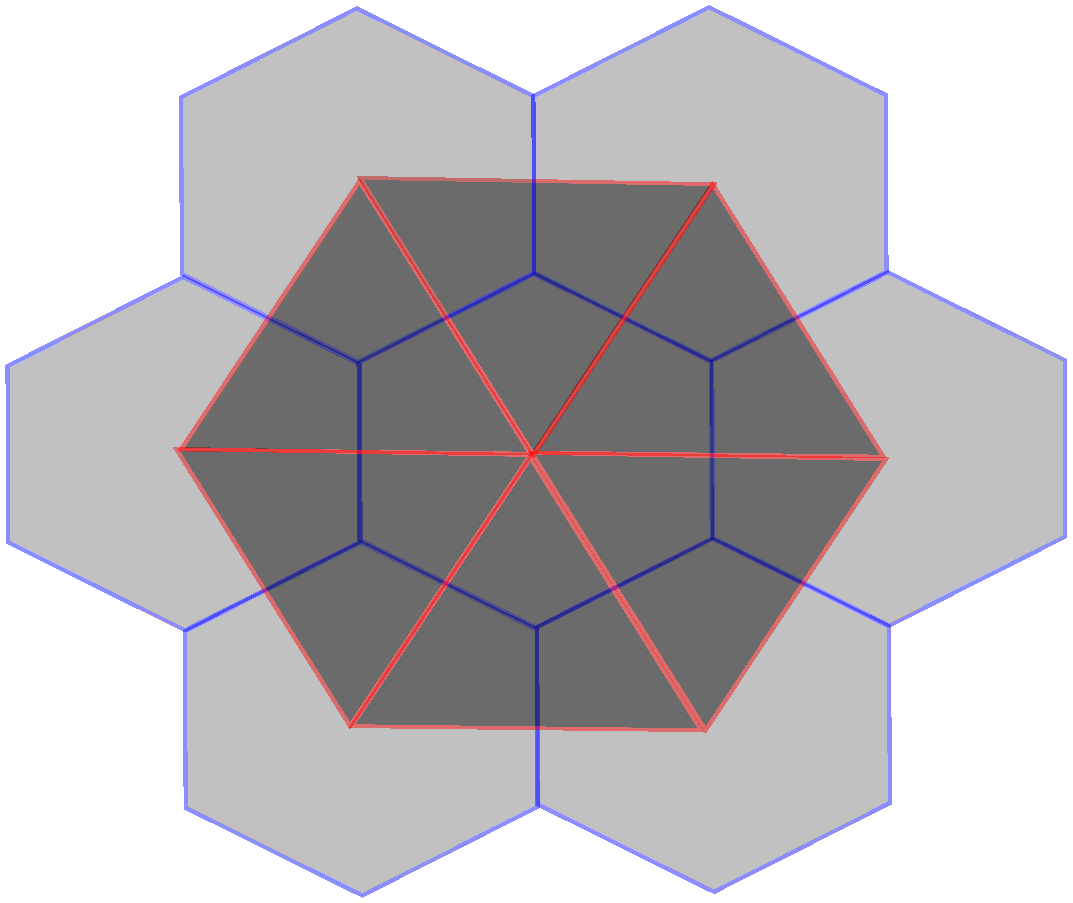
\includegraphics[width = 0.6\textwidth]{hexagonal_grid_0.pdf}
\caption{A subset of a regular horizontal hexagonal grid. The hexagonal grid (blue lines) and the triangular grid (red lines) form a pair of a primal-dual grid. In \texttt{GAME}, the hexagonal grid is the primal grid, while the triangulars form the dual one. In a triangular grid model it is the other way around. During the grid generation procedure we refer to the triangle edge points (hexagon centers) as the generating points or generators, for short.}
\label{fig:hexagonal_grid_0}
\end{center}
\end{figure}

\section{Fundamental grid quantities}
\label{sec:fundamental_grid_quantities}

The following quantities are sufficient to uniquely define the grid:

\begin{itemize}
\item the horizontal coordinates of the generating points
\item the numbering of the generating points
\item the numbering and orientation of the horizontal vectors
\item the numbering of the dual cell mid points
\item The orientation of the dual horizontal vectors. Since their horizontal positions coincide with the horizontal positions of the primal vectors, both sets of vectors can be numbered in the same way.
\end{itemize}
%
All other quantities, be it floating point numbers like grid box volumes or areas, or integer quantities like neighborhood relationships, can be implicitly derived. Consequently, once must firstly focus on the fundamental grid properties.

\subsection{Creating a spherical geodesic grid}
\label{sec:creating_a_spherical_geodesic_grid}

By \textit{horizontal grid} we mean the grid on one single layer. Without loss of generality this layer can be assumed to coincide with the surface of the unity sphere.

\subsection{Numbering and orienting the vector points}
\label{sec:numbering_and_orienting_the_vector_points}

\subsection{Numbering and orienting the dual vector points}
\label{sec:numbering_and_orienting_the_dual_vector_points}

Until now, we have only operated with the six following arrays:
%
\begin{itemize}
\item \texttt{latitude\_scalar}, \texttt{longitude\_scalar}
\item \texttt{from\_index}, \texttt{to\_index}
\item \texttt{from\_index\_dual}, \texttt{to\_index\_dual}
\end{itemize}
%

\section{Derived quantities}
\label{sec:derived_quantities}

\subsection{Horizontal coordinates of dual scalar points}
\label{sec:horizontal_coordinates_of_dual_scalar_points}

The dual cells of a hexagonal grid are the triangular grid cells. Since we aim at an orthogonal grid, the dual scalar points must be the Voronoi centers of the triangular cells. Label the vertices of one triangle with $\mathbf{r}_0, \mathbf{r}_1, \mathbf{r}_2$, then its Voronoi center $\mathbf{r}_v$ is located at the position
%
\begin{align}
\mathbf{r}_v \coloneqq \frac{\left(\mathbf{r}_1 - \mathbf{r}_0\right)\times\left(\mathbf{r}_2 - \mathbf{r}_0\right)}{\left|\left(\mathbf{r}_1 - \mathbf{r}_0\right)\times\left(\mathbf{r}_2 - \mathbf{r}_0\right)\right|}.
\end{align}

\subsection{Finding the neighboring vector points of a primal cell and their orientation}
\label{sec:finding_the_neighboring_vector_points_of_a_primal_cell_and_their_orientation}

\begin{figure}
\begin{center}
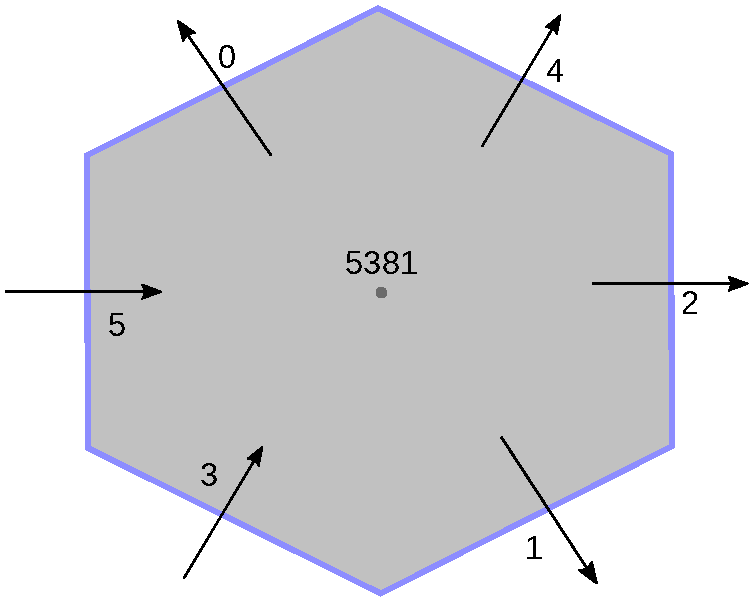
\includegraphics[width = 0.5\textwidth]{hexagonal_grid_1.pdf}
\caption{A sample hexagon with a horizontal scalar index of 5381. The directions of the arrows indicate the directions of unit vectors at cell edges. The drawn orientations would lead to $\texttt{adjacent\_vector\_signs\_h}[6\cdot 5381 + 0] = 1$, $\texttt{adjacent\_vector\_signs\_h}[6\cdot 5381 + 1] = 1$, $\texttt{adjacent\_vector\_signs\_h}[6\cdot 5381 + 2] = 1$, $\texttt{adjacent\_vector\_signs\_h}[6\cdot 5381 + 3] = -1$, $\texttt{adjacent\_vector\_signs\_h}[6\cdot 5381 + 4] = 1$, $\texttt{adjacent\_vector\_signs\_h}[6\cdot 5381 + 5] = -1$.}
\label{fig:hexagonal_grid_1}
\end{center}
\end{figure}

\subsection{Finding the neighboring vector points of a dual cell and their orientation}
\label{sec:finding_the_neighboring_vector_points_of_a_dual_cell_and_their_orientation}

\section{Grid optimization}
\label{sec:grid_optimization}

Hexagonal spherical grids need to be optimized for numerical modeling. Therefore, the Lloyd algorithm is used, which yields a \textit{spherical centroidal Voronoi tesselation (SCVT)} after convergence \cite{Du2003}. \cite{PEIXOTO201361} gives an overview of optimization alternatives and it seems to be that the SCVT is the most suitable for modeling. The procedure employed for executing the Lloyd algorithm is the one described in \cite{10.1175/MWR2991.1}.

\section{Vertical grid structure}
\label{sec:vertical_grid_structure}

So far, only a horizontal grid has been examined. The grid generator, however, shall produce full three-dimensional grids. In order to simplify matters, the following conventions are made:
%
\begin{itemize}
\item Since the vertically oriented primal vector points have the same horizontal coordinates as the primal scalar points, their horizontal numbering is also the same.
\item Since the vertically oriented dual vector points have the same horizontal coordinates as the dual scalar points, their horizontal numbering is also the same.
\end{itemize}

\section{Scalability}
\label{sec:scalability}

The computation time of the most expensive for loops scale with $N^2$, where $N$ is the number of horizontal grid points. This means that doubling the horizontal resolution (four times as much horizontal grid points) leads to a 16 times longer computation time of the grid generator. This is similar to the model itself, where a doubling of the horizontal and vertical resolution and a halfening of the time step leads to 16 times longer integration times. Therefore, the largely implicit formulation of the grid generator posos no problem to its performance at higher resoultions.

\subsection{Permutations of the grid points}
\label{sec:permutations_of_the_grid_points}

\chapter{Orography generator}
\label{sec:orography_generator}

The orography generator resides in the directory \texttt{orography\_generator} and is an individual executable meant to produce orographies for different cases defined by and \texttt{oro\_id}, given the horizontal positions of the primal scalar points.

\chapter{Prognostic and diagnostic quantities}
\label{sec:prognostic_and_diagnostic_quantities}

\chapter{Test generator}
\label{sec:test_generator}

The so-called \textit{full width at half maximum (FWHM)} is the width of a peak at half its maximum height. For a normal distribution, one finds
%
\begin{align}
\exp\left(-\frac{x_0^2}{2\sigma^2}\right) = \frac{1}{2} = 2^{-1}\Leftrightarrow -\frac{x_0^2}{2\sigma^2} = -\ln\left(2\right)\nonumber\\
\Leftrightarrow x_0^2 = 2\sigma^2\ln\left(2\right)\Leftrightarrow x_0 = \sigma\sqrt{2\ln\left(2\right)}.
\end{align}
%
This implies
%
\begin{align}
\text{FWHM} = 2x_0 = \sigma\sqrt{8\ln\left(2\right)} \Rightarrow \sigma = \frac{\text{FWHM}}{\sqrt{8\ln\left(2\right)}}.
\end{align}

\chapter{Spatial operators}
\label{sec:spatial_operators}

\begin{itemize}
\item Coriolis: \cite{thuburn_f_discrete_plane} and \cite{ringler_trsk} modified by \cite{doi:10.1002/qj.3294}
\item kinetic energy: \cite{doi:10.1002/qj.1960}
\end{itemize}

\chapter{Time stepping}
\label{sec:time_stepping}

Runge-Kutta third order scheme (RK3). In the vertical, at every substep, implicit methods are used.

\chapter{Input and output}
\label{sec:input_and_output}

\chapter{Coupling to the radiation field}
\label{chap:coupling_to_the_radiation_field}

\texttt{GAME} employs the so-called \texttt{RTE+RRTMGP (Radiative Transfer for Energetics + Rapid and Accurate Radiative Transfer Model for Geophysical Circulation Model Applications—Parallel)} \cite{doi:10.1029/2019MS001621}, \cite{rte-rrtmgp-github} scheme.

\appendix

\printbibliography

\end{document}













